\section{Introducción}

\noindent La edición 2024 de Sitevinitech, la feria más importante de la industria vitivinícola y agrícola de Latinoamérica, culminó con gran éxito el pasado 17 de mayo. Celebrada en el complejo Las Naves de la Ciudad de Mendoza, la feria reunió a más de 500 expositores de 20 países y recibió a más de 10.000 visitantes, consolidando su posición como el principal punto de encuentro para el sector vitivinícola de la región.

\section{Innovación y negocios en el centro de la escena}

La feria se caracterizó por su fuerte enfoque en la innovación y la generación de negocios. Los expositores presentaron las últimas tecnologías y soluciones para el sector, desde maquinaria y equipos hasta software y servicios. Entre las novedades más destacadas se encontraron:

\begin{itemize}
    \item \textbf{Sistemas de desalcoholización de vinos:} Estos sistemas permiten reducir el contenido de alcohol del vino sin afectar su sabor o calidad.
    \item \textbf{Máquinas para la elaboración de vinos espumosos:} Estas máquinas permiten automatizar el proceso de elaboración de vinos espumosos, lo que reduce costos y aumenta la eficiencia.
     \item \textbf{Tecnologías para el control de la calidad del vino:} Estas tecnologías permiten a los productores controlar la calidad del vino en todas las etapas de producción, desde la uva hasta la botella.
     \item \textbf{uso de drones en la vitivinicultura:} Los drones han irrumpido en la industria vitivinícola como una herramienta innovadora con un gran potencial para optimizar la producción y mejorar la rentabilidad de las bodegas. Estas aeronaves no tripuladas pueden ser equipadas con diversos sensores y cámaras que les permiten recopilar información valiosa y hasta realizar tareas como aplicación de fertilizantes.
    \item \textbf{Software de producción y gestión para bodegas:} Se ha convertido en una herramienta fundamental para optimizar las operaciones y mejorar la rentabilidad de las empresas vitivinícolas. Estos programas ofrecen una amplia gama de funcionalidades que permiten a los productores controlar el inventario, gestionar la producción, gestionar ventas y distribución, etc.
\end{itemize}
 
Además de la exposición de productos y servicios, se desarrollaron diversas actividades para promover el intercambio comercial y la creación de redes de contacto, como rondas de negocios, workshops y seminarios. Estas actividades fueron muy valoradas por los participantes, ya que les permitieron conocer nuevos proveedores, clientes y socios potenciales.

\begin{figure}[h!]
    \centering
    %Modificando los parámetros de height puedes cambiar el tamaño de tu imagen.
    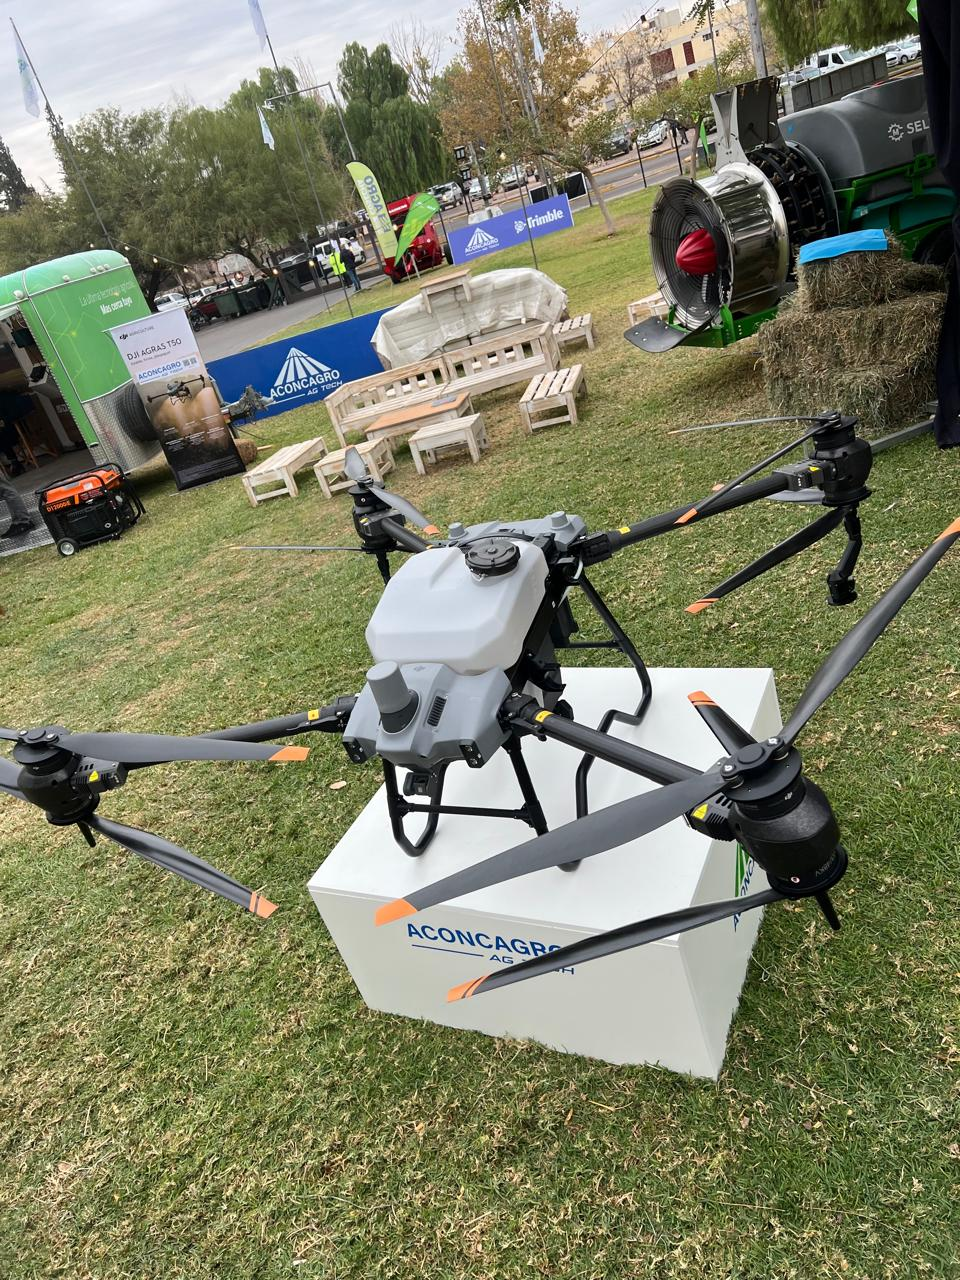
\includegraphics[height=9cm]{Imágenes/drone.jpeg}
    \caption{\textit{Drone Fumigador DJI}}
    \label{exemploLabel}
    \end{figure}

\section{Sustentabilidad y cuidado del medio ambiente}

Sitevinitech 2024 también dio gran importancia a la sustentabilidad y el cuidado del medio ambiente. Se dedicó un pabellón especial a las empresas que trabajan en el desarrollo de soluciones sostenibles para la industria vitivinícola, y se realizaron diversas actividades para concientizar sobre la importancia de la producción sostenible. Entre las iniciativas más destacadas se encontraron: 

    
\begin{itemize}
\item \textbf{Paneles solares para bodegas:} Estos paneles permiten a las bodegas generar su propia energía eléctrica, lo que reduce su impacto ambiental y les permite ahorrar dinero.
\item \textbf{Sistemas de riego por goteo:} Estos sistemas permiten utilizar el agua de manera más eficiente, lo que es especialmente importante en zonas áridas como Mendoza.
\item \textbf{Uso de envases reciclables:} Cada vez más bodegas están utilizando envases reciclables para sus vinos, lo que ayuda a reducir la cantidad de residuos que se generan.
\end{itemize}

\begin{figure}[h!]
    \centering
    %Modificando los parámetros de height puedes cambiar el tamaño de tu imagen.
    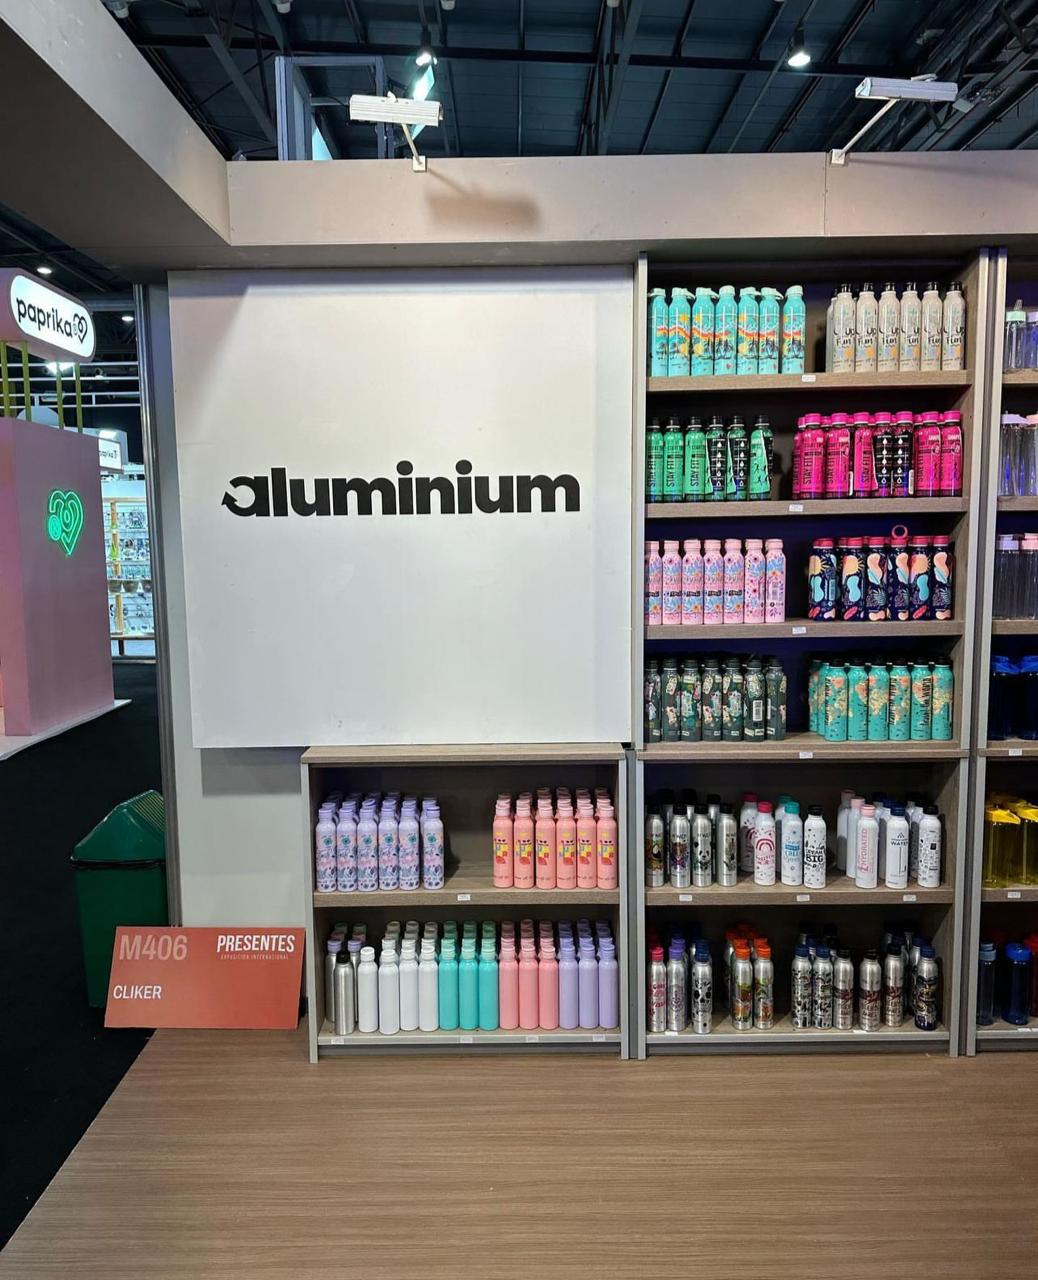
\includegraphics[height=9cm]{Imágenes/alu.jpeg}
    \caption{\textit{Botellas de aluminio reciclado para envasado de vinos}}
    \label{exemploLabel}
    \end{figure}
 
\section{Vintrace: Erin Foley}

En el siguiente apartado se expondrá sobre Vintrance una empresa que ofrece el conjunto de herramientas digitales más impresionante para la industria vitivinícola mundial.
Hablamos con Erin Foley, vicepresidente de Vintrance y encargada de gestión de productos. 
\begin{figure}[h!]
    \centering
    %Modificando los parámetros de height puedes cambiar el tamaño de tu imagen.
    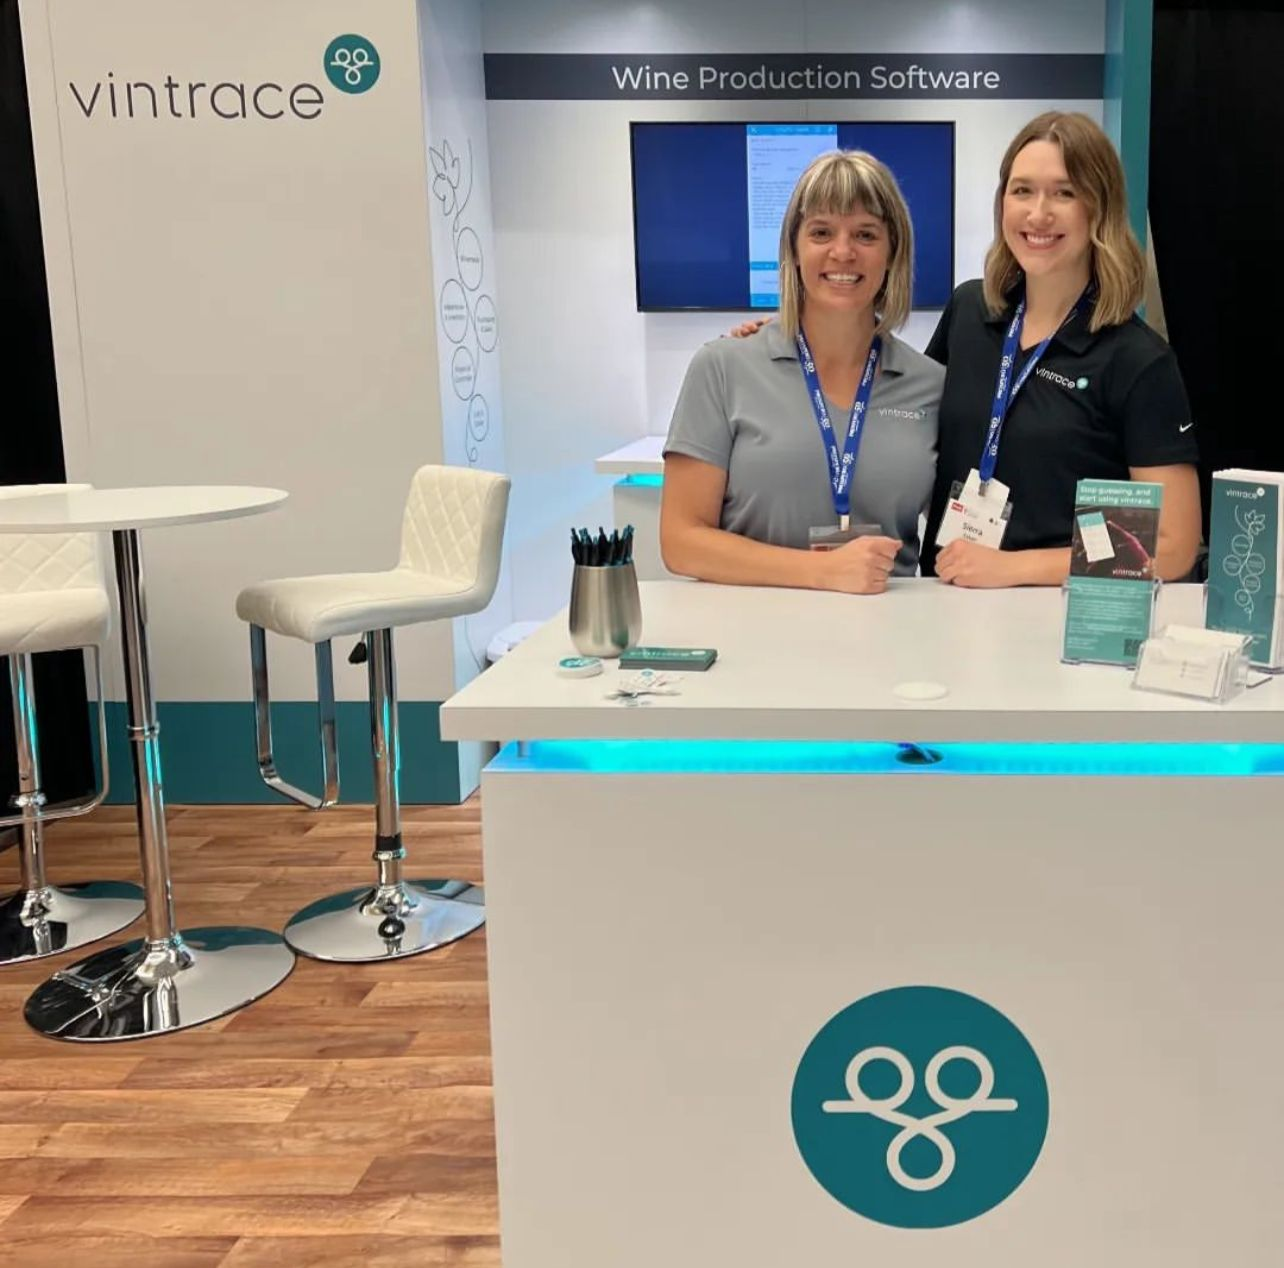
\includegraphics[height=9cm]{Imágenes/stand.jpeg}
    \caption{\textit{Estand de Vintrace en Sitevinitech 2024}}
    \label{exemploLabel}
    \end{figure}
El software de producción de vinos de Vintrace permite ahorrar tiempo para que puedas concentrarte en tu arte, colaborar con tu equipo desde cualquier sitio y obtener ideas inteligentes para una mejor toma de decisiones.
Las principales ventajas de Vintrace son:
\begin{itemize}
\item \textbf{Visibilidad completa sobre reservas de cosechas, vino y órdenes de trabajo}
\item \textbf{Visión integral de sus instalaciones con una potente función de mapeo y gestión de tanques}
\item \textbf{Capacidad de crear mezclas/blend de prueba}
\item \textbf{Aplicación móvil con accesibilidad para usuarios iOS y Android}
\item \textbf{Trazabilidad de punta a punta que cumple con los requisitos de la regulación de la seguridad alimentaria FDA HACCP}
\item \textbf{Escalabilidad para manejar múltiples locaciones, vinificaciones personalizadas, programas de espumosos, su creciente fuerza laboral, gestión DSP (Destilería) y mucho más}
\end{itemize}
 \begin{figure}[h!]
    \centering
    %Modificando los parámetros de height puedes cambiar el tamaño de tu imagen.
    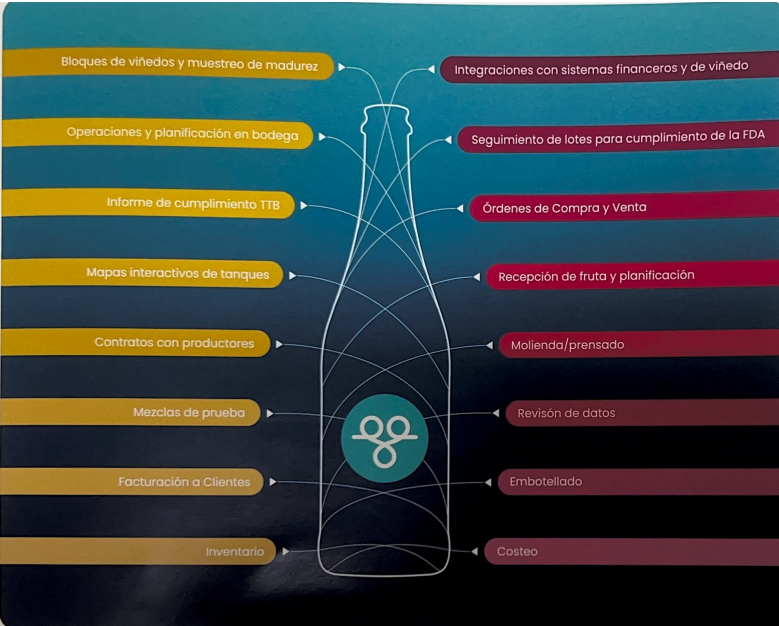
\includegraphics[height=9cm]{Imágenes/agd.png}
    \caption{\textit{Presentación de funciones de Vintrace}}
    \label{exemploLabel}
    \end{figure}

    
\section{Utilización de Vintrace antes, durante y después de la cosecha}
Desde la planificación previa, hasta el análisis posterior de la cosehca, Vintrace ofrece beneficios significativos para bodegas de todo el mundo. El poder combinado de enólogos y el soporte de Vintrace crea posibilidades de control y planificación permitiendo que cada etapa de producción fluya.

 \begin{figure}[h!]
    \centering
    %Modificando los parámetros de height puedes cambiar el tamaño de tu imagen.
    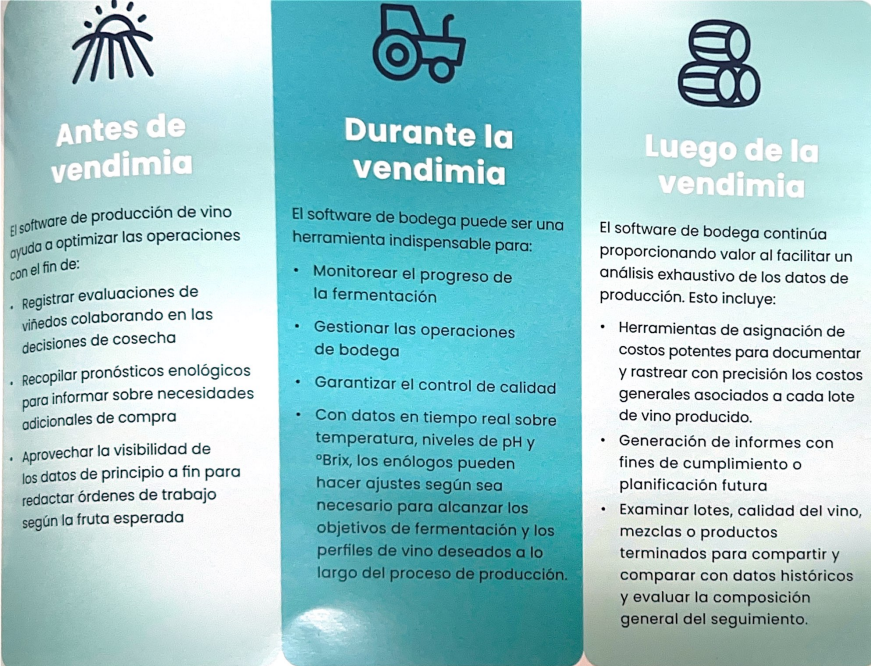
\includegraphics[height=9cm]{Imágenes/vendimia.png}
    \caption{\textit{Utilizando Vintrace antes, durante y después de la cosecha}}
    \label{exemploLabel}
    \end{figure}
Vintrace no solo optimiza las operaciones individuales, sino que integra la gestión de todo el proceso de elaboración del vino, desde la recepción de la uva hasta el embotellado y la distribución. Esta visión holística permite a las bodegas identificar y eliminar cuellos de botella, mejorar la eficiencia en todos los niveles y garantizar la calidad constante del producto final.

Empoderamiento a través de la toma de decisiones basada en datos:

Vintrace proporciona a las bodegas acceso a una gran cantidad de datos en tiempo real sobre cada etapa del proceso de producción. Estos datos, recopilados automáticamente a través de sensores y registros manuales, se consolidan en un único panel de control intuitivo, brindando a los enólogos y gerentes la información que necesitan para tomar decisiones acertadas y oportunas.

Beneficios tangibles para las bodegas:
\begin{itemize}
\item \textbf{Mayor eficiencia:}Reducción de tiempos de ciclo, disminución de desperdicios y optimización del uso de recursos.
\item \textbf{Calidad superior del vino:}Control preciso de la temperatura, la fermentación y otros parámetros críticos para obtener vinos excepcionales.
\item \textbf{Mejora en los resultados comerciales:}Aumento de la productividad, reducción de costos y mayor rentabilidad.
\end{itemize}



\section{Conclusion}
Finalmente, concluimos que Vintrace se presenta como una herramienta integral para la gestión del proceso de elaboración del vino, desde la uva hasta la botella. A través de la optimización de operaciones, el empoderamiento de la toma de decisiones basada en datos y la consecución de resultados tangibles, Vintrace se posiciona como un aliado estratégico para las bodegas.
Avalado por casos de éxito en Estados Unidos, Canada, Australia, Nuevza Zelanda y buscando posicionares en Argentina, Vintrace se perfila como una herramienta indispensable para las bodegas que buscan alcanzar el éxito a largo plazo.
Nos pareció una herramienta muy interesante e innovadora para incorporar en las bodegas de Mendoza.


\begin{figure}[h!]
    \centering
    %Modificando los parámetros de height puedes cambiar el tamaño de tu imagen.
    
\includegraphics[height=9cm]{Imágenes/vintrace.png}
    \caption{\textit{Logo Vintrace}}
    \label{exemploLabel}
    \end{figure}